%Version 3 December 2023
% See section 11 of the User Manual for version history
%
%%%%%%%%%%%%%%%%%%%%%%%%%%%%%%%%%%%%%%%%%%%%%%%%%%%%%%%%%%%%%%%%%%%%%%
%%                                                                 %%
%% Please do not use \input{...} to include other tex files.       %%
%% Submit your LaTeX manuscript as one .tex document.              %%
%%                                                                 %%
%% All additional figures and files should be attached             %%
%% separately and not embedded in the \TeX\ document itself.       %%
%%                                                                 %%
%%%%%%%%%%%%%%%%%%%%%%%%%%%%%%%%%%%%%%%%%%%%%%%%%%%%%%%%%%%%%%%%%%%%%

%%\documentclass[referee,sn-basic]{sn-jnl}% referee option is meant for double line spacing

%%=======================================================%%
%% to print line numbers in the margin use lineno option %%
%%=======================================================%%

%%\documentclass[lineno,sn-basic]{sn-jnl}% Basic Springer Nature Reference Style/Chemistry Reference Style

%%======================================================%%
%% to compile with pdflatex/xelatex use pdflatex option %%
%%======================================================%%

%%\documentclass[pdflatex,sn-basic]{sn-jnl}% Basic Springer Nature Reference Style/Chemistry Reference Style


%%Note: the following reference styles support Namedate and Numbered referencing. By default the style follows the most common style. To switch between the options you can add or remove “Numbered” in the optional parenthesis. 
%%The option is available for: sn-basic.bst, sn-vancouver.bst, sn-chicago.bst%  
 
%%\documentclass[pdflatex,sn-nature]{sn-jnl}% Style for submissions to Nature Portfolio journals
%%\documentclass[pdflatex,sn-basic]{sn-jnl}% Basic Springer Nature Reference Style/Chemistry Reference Style
\documentclass[pdflatex,sn-mathphys-num]{sn-jnl}% Math and Physical Sciences Numbered Reference Style 
%%\documentclass[pdflatex,sn-mathphys-ay]{sn-jnl}% Math and Physical Sciences Author Year Reference Style
%%\documentclass[pdflatex,sn-aps]{sn-jnl}% American Physical Society (APS) Reference Style
%%\documentclass[pdflatex,sn-vancouver,Numbered]{sn-jnl}% Vancouver Reference Style
%%\documentclass[pdflatex,sn-apa]{sn-jnl}% APA Reference Style 
%%\documentclass[pdflatex,sn-chicago]{sn-jnl}% Chicago-based Humanities Reference Style

%%%% Standard Packages
%%<additional latex packages if required can be included here>

\usepackage{graphicx}%
\usepackage{multirow}%
\usepackage{amsmath,amssymb,amsfonts}%
\usepackage{amsthm}%
\usepackage{mathrsfs}%
\usepackage[title]{appendix}%
\usepackage{xcolor}%
\usepackage{textcomp}%
\usepackage{manyfoot}%
\usepackage{booktabs}%
\usepackage{algorithm}%
\usepackage{algorithmicx}%
\usepackage{algpseudocode}%
\usepackage{listings}%
\usepackage{braket}
\usepackage{subcaption}
\usepackage{indentfirst}

\usepackage{fancyhdr,lastpage}
\fancypagestyle{fancy}{
    \fancyhf{}
    \fancyhead[C]{QC Master @ UPB - Research Report 2}
    \fancyfoot[L]{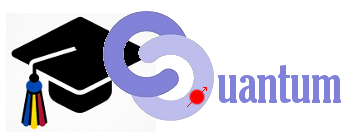
\includegraphics[scale=0.2,trim=0 0 0 -6cm]{MScQCLogo.png}}
    \fancyfoot[R]{\thepage\ of\ \pageref{LastPage}}
}

%%%%

%%%%%=============================================================================%%%%
%%%%  Remarks: This template is provided to aid authors with the preparation
%%%%  of original research articles intended for submission to journals published 
%%%%  by Springer Nature. The guidance has been prepared in partnership with 
%%%%  production teams to conform to Springer Nature technical requirements. 
%%%%  Editorial and presentation requirements differ among journal portfolios and 
%%%%  research disciplines. You may find sections in this template are irrelevant 
%%%%  to your work and are empowered to omit any such section if allowed by the 
%%%%  journal you intend to submit to. The submission guidelines and policies 
%%%%  of the journal take precedence. A detailed User Manual is available in the 
%%%%  template package for technical guidance.
%%%%%=============================================================================%%%%

\begin{document}
\pagestyle{fancy}
\thispagestyle{fancy}
\title{Generic Implementation of the Quantum Lattice Boltzmann Method for Arbitrary Velocity Sets}
%%=============================================================%%
%% GivenName	-> \fnm{Joergen W.}
%% Particle	-> \spfx{van der} -> surname prefix
%% FamilyName	-> \sur{Ploeg}
%% Suffix	-> \sfx{IV}
%% \author*[1,2]{\fnm{Joergen W.} \spfx{van der} \sur{Ploeg} 
%%  \sfx{IV}}\email{iauthor@gmail.com}
%%=============================================================%%

\author*[1]{\fnm{Andrei} \sur{Tavă}}\email{andrei\_daniel.tava@stud.acs.upb.ro}

\affil*[1]{\orgdiv{Computer Science and Engineering Department}, \orgname{University Politehnica of Bucharest}, \orgaddress{\city{Bucharest}, \country{Romania}}}

%%==================================%%
%% Sample for unstructured abstract %%
%%==================================%%

\abstract{
    This report presents a fully generic and parameterized implementation of the Quantum Lattice Boltzmann Method for the advection-diffusion equation.
    The algorithm is based on existing work with slight modifications to the initialization procedure, but unlike all other existing implementations, ours is designed to be flexible and can handle any number of dimensions and arbitrary sets of link velocities, including non-standard sets.
    We validate our work with various experiments of increasing complexity, demonstrating that it matches classical simulations within a reasonable error margin.
}

%%================================%%
%% Sample for structured abstract %%
%%================================%%

% \abstract{\textbf{Purpose:} The abstract serves both as a general introduction to the topic and as a brief, non-technical summary of the main results and their implications. The abstract must not include subheadings (unless expressly permitted in the journal's Instructions to Authors), equations or citations. As a guide the abstract should not exceed 200 words. Most journals do not set a hard limit however authors are advised to check the author instructions for the journal they are submitting to.
% 
% \textbf{Methods:} The abstract serves both as a general introduction to the topic and as a brief, non-technical summary of the main results and their implications. The abstract must not include subheadings (unless expressly permitted in the journal's Instructions to Authors), equations or citations. As a guide the abstract should not exceed 200 words. Most journals do not set a hard limit however authors are advised to check the author instructions for the journal they are submitting to.
% 
% \textbf{Results:} The abstract serves both as a general introduction to the topic and as a brief, non-technical summary of the main results and their implications. The abstract must not include subheadings (unless expressly permitted in the journal's Instructions to Authors), equations or citations. As a guide the abstract should not exceed 200 words. Most journals do not set a hard limit however authors are advised to check the author instructions for the journal they are submitting to.
% 
% \textbf{Conclusion:} The abstract serves both as a general introduction to the topic and as a brief, non-technical summary of the main results and their implications. The abstract must not include subheadings (unless expressly permitted in the journal's Instructions to Authors), equations or citations. As a guide the abstract should not exceed 200 words. Most journals do not set a hard limit however authors are advised to check the author instructions for the journal they are submitting to.}

\keywords{Quantum Lattice Boltzmann Method, Quantum Computational Fluid Dynamics, Advection-Diffusion Equation, Quantum Algorithms, Qiskit}

%%\pacs[JEL Classification]{D8, H51}

%%\pacs[MSC Classification]{35A01, 65L10, 65L12, 65L20, 65L70}

\maketitle
\pagestyle{fancy}

\section{Introduction}
\textbf{Quantum Computational Fluid Dynamics} is a field that has seen plenty of activity in recent years \cite{gaitan2020finding, meng2023quantum, jaksch2023variational}. 
Because of the computational demands of fluid simulations, we consider that achieving quantum advantage would be a significant breakthrough.

Among the various explored methods, the \textbf{Quantum Lattice Boltzmann Method} (QLBM) is seen as a promising candidate with several groups actively researching it \cite{budinski2021quantum,itani2024quantum,kocherla2024fully, xu2025improved, tiwari2025algorithmic,wawrzyniak2025base}.
Despire theoretical advantages, there are plenty of practical challenges that need to be addressed before this method can be useful for large scale simulations, which is the area most of the research is focused on.

In this work, we present a fully generic and parameterized implementation of a QLBM algorithm for the \textbf{advection-diffusion equation}.
As of writing and to the best of our knowledge, this is the only such implementation available.

\subsection{The Quantum Lattice Boltzmann Method}
The QLBM, as the name suggests, is the quantum version of the classical Lattice Botlzmann Method (LBM) algorithm.

LBMs work by discretizing space into a lattice structure, where each lattice site contains a set of \textbf{link distributions}.
Each link distribution has an associated link velocity and represents the proportion of the simulated quantity that will propagate along that link.
Discretization schemes are named after the number of dimensions and the number of links: D1Q3 for 1D with 3 links D2Q9 for 2D with 9 links, D3Q27 for 3D with 27 links.

\begin{figure}[h]
    \begin{center}
    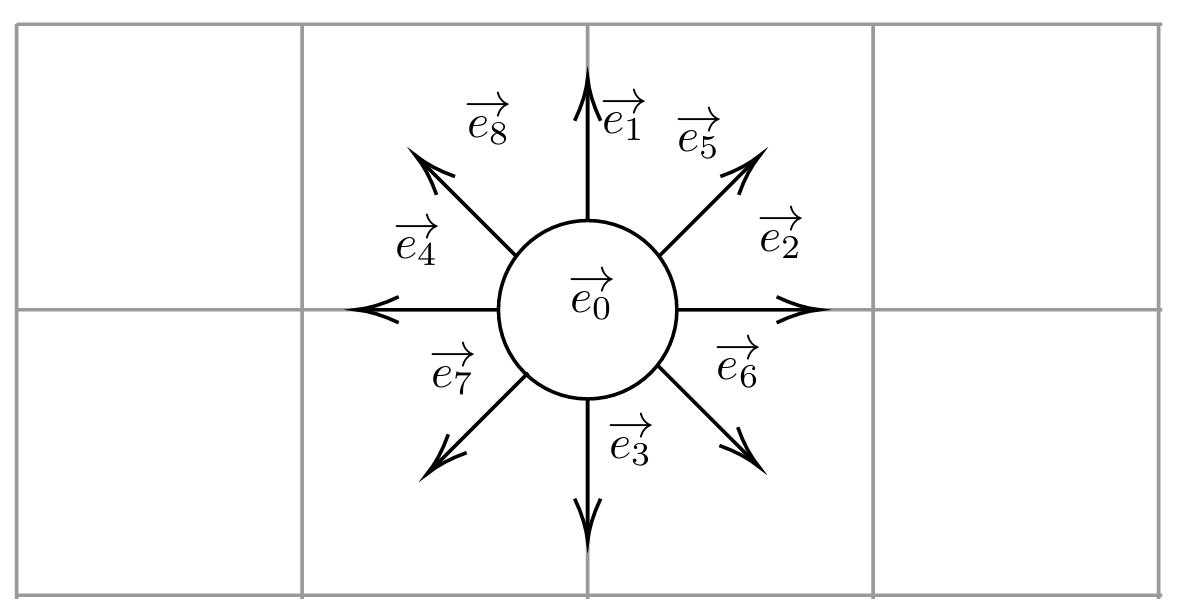
\includegraphics[width=0.5\textwidth]{figures/lbm.png}
    \end{center}
    \caption{D2Q9: 2D lattice with 9 discrete velocities.}
    \label{fig:disc}
\end{figure}


An iteration of the algorithm consists of two main steps:
\begin{enumerate}
    \item \textbf{Collision:} The values of the link distributions are updated based on a \textbf{collision operator}. The specific operator depends on details of the simulated behavior.
    \item \textbf{Streaming:} The distribution values are propagated to neighboring sites based on the defined link velocities.
\end{enumerate}

Finally, the link distributions are summed up in order to recover the macroscopic distribution.

One of the earliest implementations of a QLBM was proposed by Boudinski \cite{budinski2021quantum}.
He proposed a quantum circuit that could simulate flows governed by the \textbf{advection-diffusion equation}:

\begin{equation}
    \partial_t\Phi = D\nabla^{2}\Phi - \nabla(\mathbf{u}\Phi)
\end{equation}

Where $\Phi(x)$ is the distribution function, $D$ is the diffusion coefficient and $\mathbf{u(x)}$ is the velocity field.

He later extended the method to the Navier-Stokes equations \cite{ljubomir2022quantum} via the stream-vorticity formulation and validated his results in a lid-driven cavity flow simulation.

\section{Algorithm Implementation}
Our QLBM algorithm is based on the work of Wawrzyniak et al. \cite{wawrzyniak2025base}, which in turn builds upon Boudinski's original algorithm.
Their version extends the original algorithm to support nonuniform velocity fields and improves the initialization procedure.

For the algorithm itself, our contribution is simplyfing the initialization thus slightly reducing the gate count, at the cost of minor numerical differences. The gate count reduction is linear in the number of links.

Unlike all previous implementations we could find, we provide a trully generic, parameterized implementation that can work with any number of dimensions and any arbitrary set of links, including non-standard sets.
For the implementation we used the Qiskit framework and the Qiskit Aer Statevector simulator \cite{qiskit2024}.

An iteration of the algorithm consists of 4 steps:
\begin{enumerate}
    \item Initialization: Prepare the quantum state with the initial distribution function.
    \item Collision: Apply the collision operator to update the link distributions.
    \item Streaming: Propagate the link distributions to neighboring sites based on the link velocities.
    \item Compute macros: Recover the macroscopic distribution from the final state.
\end{enumerate}

Performing multiple iterations requires reinitializing the quantum state with the updated distribution function after each iteration.
If the velocity field or the link velocities change between iterations, the quantum circuit must be reconfigured accordingly.

\begin{figure}[H]
    \centering
    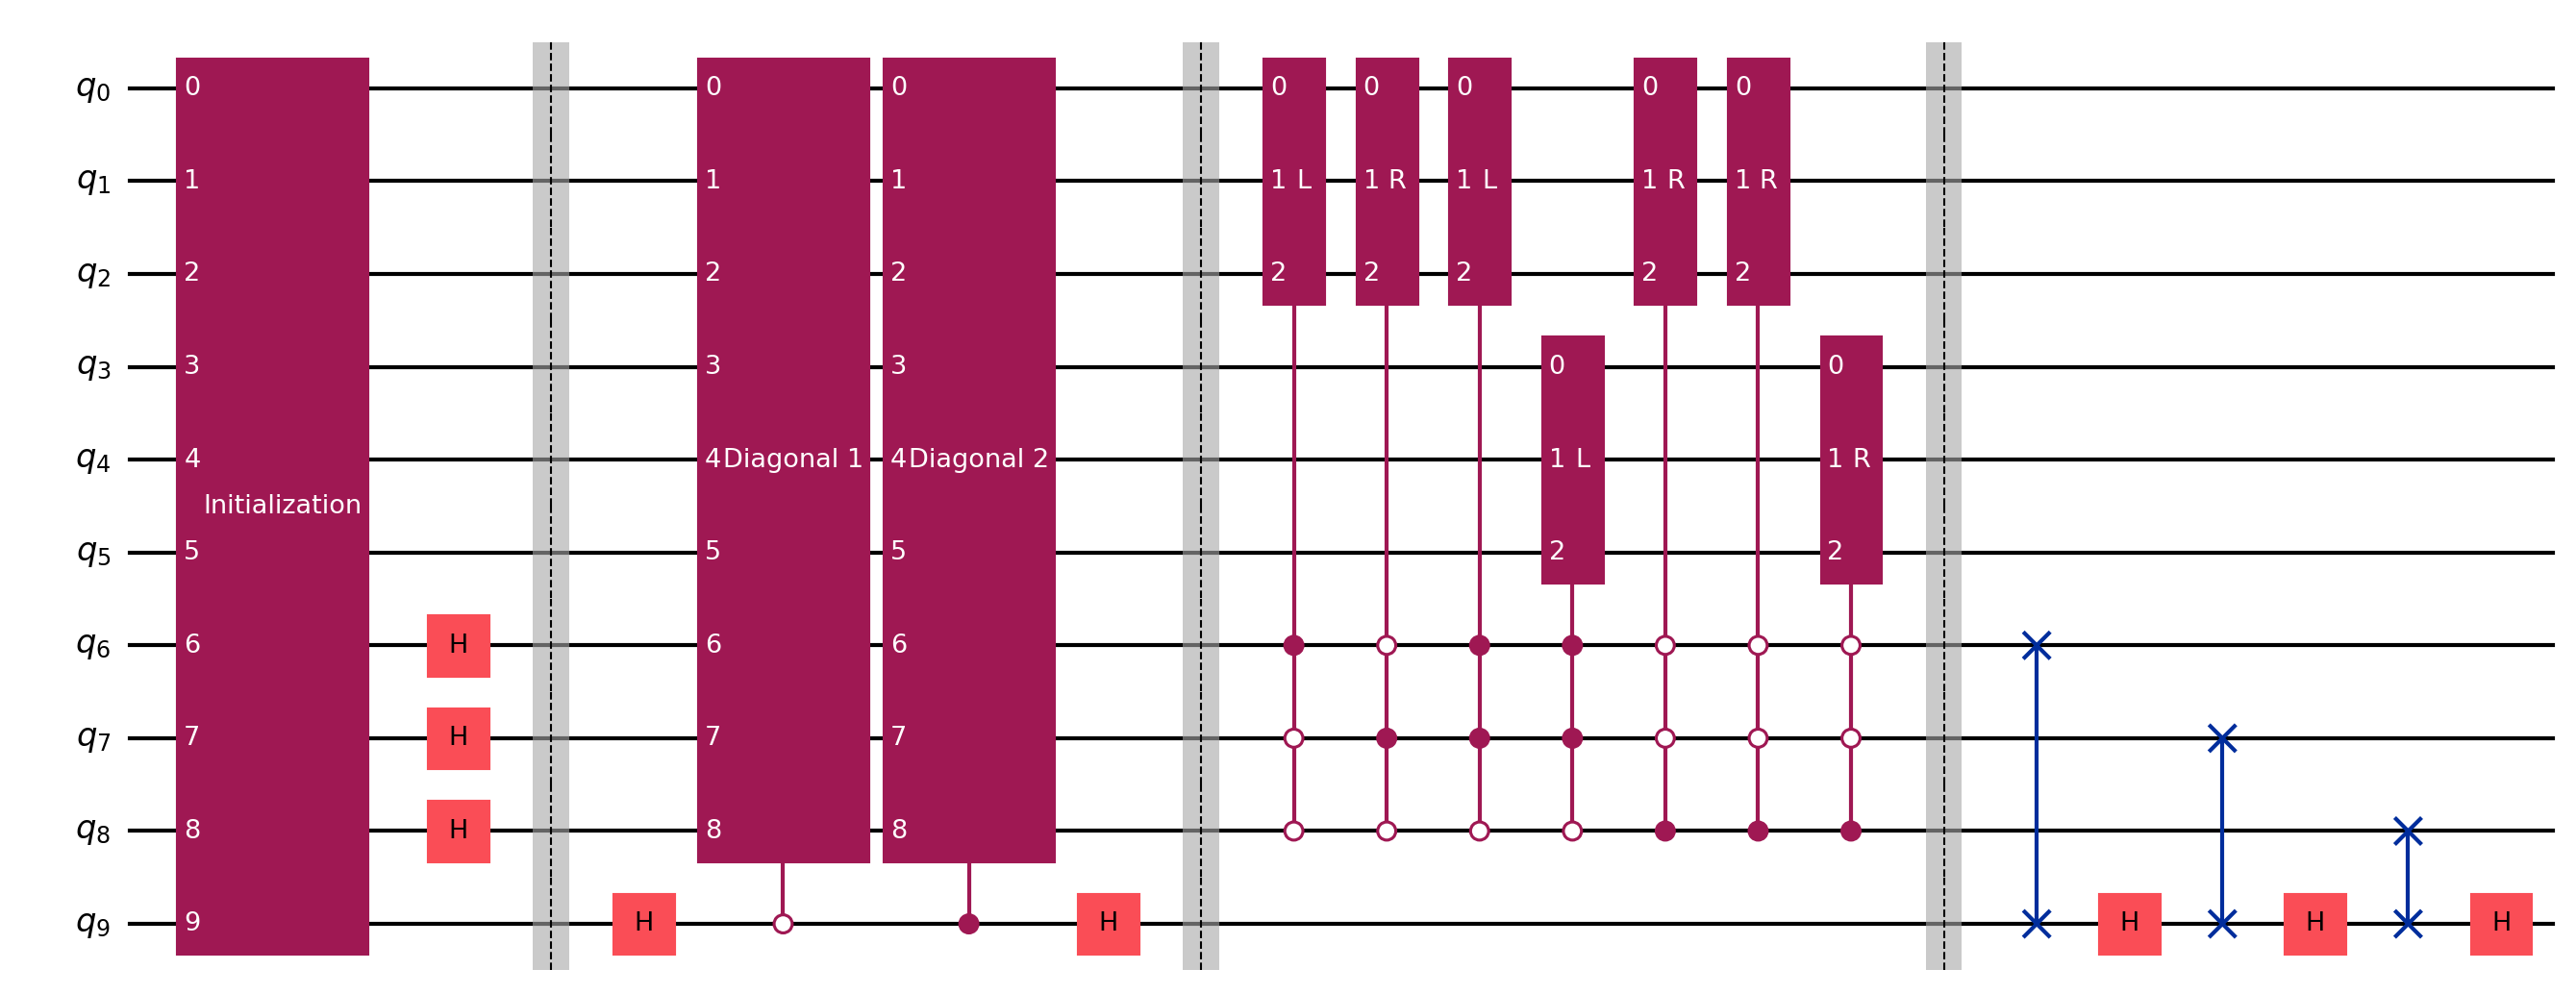
\includegraphics[width=\textwidth]{figures/complete_circuit.png}
    \caption{Complete quantum circuit for a single iteration of the QLBM algorithm. $q_{0-2}$ encode the X dimension, $q_{3-5}$ encode the Y dimension, $q_{6-8}$ encode the link velocities and $q_{9}$ is the ancilla qubit. The circuit is parameterized by the link velocities $[(0,0), (-1,0), (1,0), (-1,-1), (2,1)]$}
    \label{fig:complete_circuit}
\end{figure}


\subsection{Initialization}
The distribution function is flatened and encoded as amplitudes of a quantum state.
The number of qubits required for the total state is:
\begin{itemize}
    \item $n = \lceil \log_2(N) \rceil$, where $N$ is the number of links.
    \item $m = \sum_{i} \lceil \log_2(M_i) \rceil$, where $M_i$ is the number of lattice sites in dimension $i$.
    \item 1 ancilla qubit required for the Collision step.
\end{itemize}

The resulting state is:

\begin{equation}
    \ket{\psi} = \ket{0}\ket{0}^n\sum_{x} \frac{\Phi(x)}{||\Phi(x)||} \ket{x}
\end{equation}

Where the first qubit is the ancilla, the next $n$ qubits encode the link index and the remaining $m$ qubits encode the lattice site index.
The initialization is performed via Qiskit's \texttt{initialize} function, which makes use of Iten et al.'s exponential procedure \cite{iten2016isometries} to prepare a state given arbitrary amplitudes.

Following Wawrzyniak et al., we only initialize one of the link substates like this and make use of Hadamard gates to prepare the remaining substates.
Unlike them however, we do not attempt to only initialize the $N$ link substates, but instead initialize the entire link subspace as an equal superposition.

\begin{equation}
    \ket{\psi} = \ket{0}\frac{1}{\sqrt{2^n}}\sum_{i}^{2^n} \ket{i}\sum_{x}\frac{\Phi(x)}{||\Phi(x)||} \ket{x}
\end{equation}

The extra states are handled by the collision operator which will update them to zero.
This choice reduces the gate count and simplifies the implementation.

\subsection{Collision}
Approximating the Advection Diffusion equation using the LBM discretization and using the Bhatnagar-Gross-Krook (BGK) collision operator \cite{bhatnagar1954model}, we can express the collision step as:
\begin{equation}
    \Phi_i(x,t) = w_i \Phi_i(x,t)(1 + \frac{\mathbf{e}_i \cdot \mathbf{u}(\mathbf{x},t)}{c_s^2})
\end{equation}

With $w_i$ being the link weight, $\mathbf{e}_i$ the link velocity, $\mathbf{u}(\mathbf{x},t)$ the velocity field at site $\mathbf{x}$ and time $t$ and $c_s$ the speed of sound.

This operation can be implemented as a diagonal matrix $M$ of size  $2^{m+n} \times 2^{m+n}$, where $m$ is the number of lattice qubits and $n$ is the number of link qubits.

Unfortunately, this matrix is not unitary, but we can circumvent this by using a technique called \textbf{Linear Combination of Unitaries} \cite{childs2012hamiltonian}.
We can express $M$ as $\frac{1}{2}(U_1 + U_2)$ with $U_1 = M + i\sqrt{I - M^2}$ and $U_2 = M - i\sqrt{I - M^2}$.

These matrices are both unitary and can be implemented as quantum gates.
We used qiskit's \texttt{DiagonalGate} to implement these unitaries, which defines a gate by a diagonal matrix.

To apply the desired linear combination, we utilize an ancilla qubit prepared in the state $\ket{0} + \ket{1}$.
Then we apply each of the unitaries conditioned on the $\ket{0}$ and $\ket{1}$ states of the ancilla qubit, respectively.
Other than the ancilla, the drawback of this method is that our desired result is only present in the $\ket{0}$ substate.
This is not a problem when performing Statevector simulations, but it increases the number of shots required for running the algorithm on a real quantum computer.

\subsection{Streaming}
Streaming involves propagating the link distributions to neighboring sites based on the link velocities.
The basic operation is shifting the amplitudes of a quantum state left or right, denoted as $L\_Gate$ and $R\_Gate$ respectively.

\begin{figure}[H]
    \centering
    \begin{subfigure}[b]{0.45\textwidth}
        \centering
        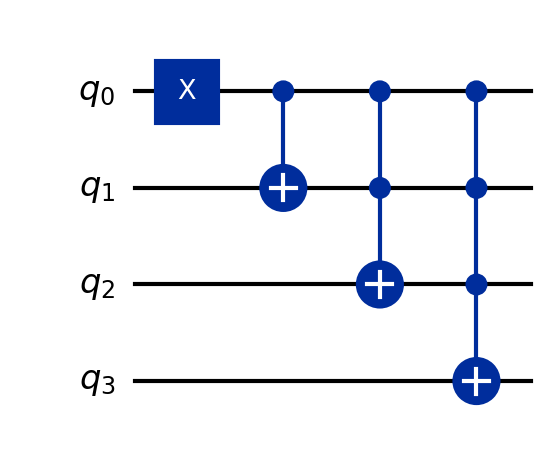
\includegraphics[width=\textwidth]{figures/l_gate.png}
        \caption{$L\_Gate$ for 4 qubits}
        \label{fig:l_gate}
    \end{subfigure}
    \hfill
    \begin{subfigure}[b]{0.45\textwidth}
        \centering
        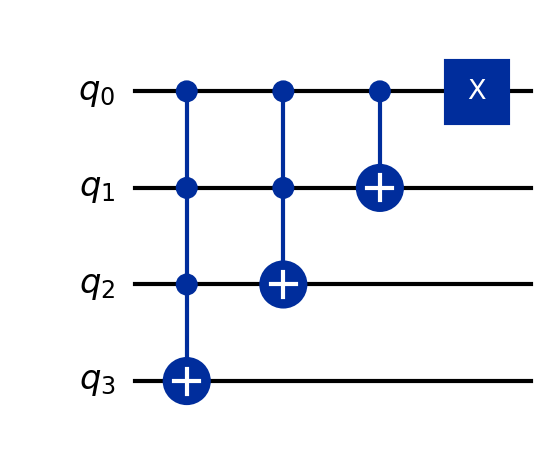
\includegraphics[width=\textwidth]{figures/r_gate.png}
        \caption{$R\_Gate$ for 4 qubits}
        \label{fig:r_gate}
    \end{subfigure}
    \caption{Quantum circuits for implementing the streaming operation}
    \label{fig:streaming_gates}
\end{figure}

Conditionally applying these gates based on the binary encoding of the link index allows us to propagate the link distributions for any arbitraty link velocity vector.
For example, to perform streaming by the velocity vector $(2,-1)$, we would apply the $R\_Gate$ twice to the qubits encoding the first dimension and the $L\_Gate$ once to the qubits encoding the second dimension.

\subsection{Computing Macros}

Finally, we need to recover the macroscopic distribution by summing over the link distributions.
This can be done both classically, after obtaining the final state or by applying a series of Hadamard and Swap gates to accumulate the distributions into a single link substate.

Our implementation provides both options.

\section{Experiments}
To validate our implementation, we performed a series of experiments with various configurations and compare the results against classical simulations.
\begin{itemize}
    \item A 1D simulation with a constant velocity field
    \item A 2D simulations with a non-uniform velocity field
    \item A 3D simulation with a non-uniform velocity field
    \item A 2D simulation with non-uniform, time-varying velocity field and non-standard link velocities.
\end{itemize}
For details on the specific configurations that might be omited, please refer to the code repository.
The full RMSE plots for all experiments are available in Appendix \ref{app:rmse}.

\subsection{1D Simulation}
THe QLBM configuration used was a standard 1DQ3 with 32 lattice sites.
The initial distribution is a simple Gaussian hill and the velocity field is a constant $u=0.3$

\begin{figure}[H]
    \centering
    
\includegraphics[width=\textwidth]{figures/1_Dcomparison.png}
    \caption{Comparison of quantum and classical simulations for the 1D case}
    \label{fig:1d_comparison}
\end{figure}

This experiment showed exact agreement between the quantum and classical simulations, with the RMSE in the order of $10^{-13}$ attributed to numerical errors.

\subsection{2D Simulation}
The QLBM configuration used was a standard 2DQ9 with 32x16 lattice sites.
The initial distribution is a ring of higher density and the velocity field consists of constant $u = 0.2$ in the bottom half and $u=-0.2$ in the top half with a constant $v=0.1$.

\begin{figure}[H]
    \centering
    \includegraphics[width=\textwidth]{figures/2_DQuantum.png}
    \caption{Heatmap evolution of the 2D simulation with non-uniform velocity field}
    \label{fig:2d_snapshots}
\end{figure}

Once again, the numerical differences are negligible at $10^{-13}$.

\subsection{3D Simulation}
The QLBM configuration used was a standard 3DQ27 with 8x8x8 lattice sites.
The initial distribution is three perpendicular planes of higher density and the velocity field follows the pattern:

\begin{align}
    u(x,y,z) &= A \cos(ax)\sin(by)\sin(cz) \\
    v(x,y,z) &= B \sin(ax)\cos(by)\sin(cz) \\
    w(x,y,z) &= C \sin(ax)\sin(by)\cos(cz)
\end{align}

With $A=B=C=0.2$ as the velocity amplitudes and $a=b=c=1.0$ as the spatial frequencies.

\begin{figure}[H]
    \centering
    
\includegraphics[width=\textwidth]{figures/3_Dquantum_snapshots.png}
    \caption{Isosurface evolution of the 3D simulation with non-uniform velocity field}
    \label{fig:3d_snapshots}
\end{figure}
The RMSE for this simulation is considerably higher at around $10^{-5}$, but still within acceptable limits.
This is attributed to the more complex velocity field.

\subsection{2D Simulation with Non-Standard Link Velocities}
The number of lattice sites is 32x32.
The initial distribution is a cross of higher density.

The configuration changes during the simulation in the following manner:
\begin{itemize}
    \item For the first 15 iterations, the standard 2DQ9 link velocities are used and the velocity field is a clockwise rotation vortex of magnitude $u=0.5$.
    \item For the next 10 iterations, the velocity field disappears and the link velocities are changed to the non-standard set $[(0,0), (2,1), (-2,-1)]$, restricting propagation to a single diagonal direction.
\end{itemize}

\begin{figure}[H]
    \centering
    
\includegraphics[width=\textwidth]{figures/cross_quantum_snapshots.png}
    \caption{Heatmap evolution of the 2D simulation with time-varying velocity field and non-standard link velocities}
    \label{fig:cross_snapshots}
\end{figure}

This simulation shows the highest RMSE of around $10^{-4}$. The more interesting part is that once the velocity field disappears at $t=15$, the error starts to decrease, as seen in Appendix \ref{app:rmse}.
This supports the hipothesis that the error is due to complex velocity fields.

\section{Conclusion}
In this work we presented a fully generic and parameterized implementation of a QLBM algorithm for the advecttion-diffusion equation.
We validated the implementation with various experiments of increasing complexity and demonstrated that it matches classical simulation within a reasonable error margin.

For future work, there are several directions to explore:
\begin{itemize}
    \item It is still unclear if the higher error for complex velocity fields is due to the algorithm itself or our implementation. Further investigation is required.
    \item The algorithm requires quantum state tomography at each iteration which is a crippling limitation for practical usage.
There is active research in this area, such as the work of Kocherla et al. \cite{kocherla2024fully}, in which they can defer measurement until the end of the simulation.
Combining their approach with our implementation is an interesting avenue.
    \item Both the initialization procedure and the collision operator are highly inefficient, relying on qiskit's transpiler to generate complex and deep circuits.
    \item The algorithm could be extended to simulate Navier-Stokes flows by using the stream-vorticity formulation, as proposed by Ljubomir et al. \cite{ljubomir2022quantum}.
\end{itemize}
\backmatter

\bmhead{Supplementary information}
All code is available on GitHub at \url{https://github.com/widdrr/qlbm}.

\bibliography{sn-bibliography}

\clearpage
\begin{appendices}

\section{RMSE Plots}\label{app:rmse}
This section contains the Root Mean Square Error (RMSE) plots for all experiments conducted. The RMSE is calculated between the quantum and classical simulations at each timestep.

\begin{figure}[H]
    \centering
    
\includegraphics[width=0.8\textwidth]{figures/1_Drmse_plot.png}
    \caption{RMSE plot for 1D Gaussian with constant velocity field}
    \label{fig:rmse1d}
\end{figure}

\begin{figure}[H]
    \centering
    
\includegraphics[width=0.8\textwidth]{figures/2_Drmse_plot.png}
    \caption{RMSE plot for 2D with non-uniform velocity field}
    \label{fig:rmse2d}
\end{figure}

\begin{figure}[H]
    \centering
    
\includegraphics[width=0.8\textwidth]{figures/3_Drmse_plot.png}
    \caption{RMSE plot for 3D planes with non-uniform velocity field}
    \label{fig:rmse3d}
\end{figure}

\begin{figure}[H]
    \centering
    
\includegraphics[width=0.8\textwidth]{figures/cross_rmse_plot.png}
    \caption{RMSE plot for 2D flow with time-varying velocity field and non-standard link velocities}
    \label{fig:rmsecross}
\end{figure}

\end{appendices}

\end{document}
